\documentclass{beamer}
\usetheme{default}

\usepackage{tikz}
\usetikzlibrary{positioning}

\begin{document}

\begin{frame}{Graph rewriting}

Types of transformations
\begin{itemize}
	\item adding nodes
	\item removing nodes
	\item adding/removing edges
\end{itemize}

\end{frame}

\begin{frame}{Rewrite rules}

Transformations are specified by rewrite rules.

\begin{figure}
\centering
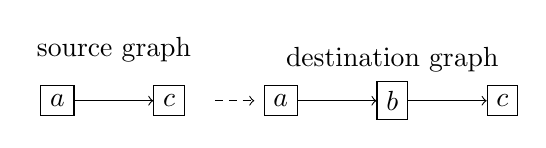
\begin{tikzpicture}

\node[draw,rectangle] (1) {$a$};
\node[draw,rectangle] (2) [right=of 1] {$c$};

\path[->]
(1) edge node[label={[label distance=0.25cm]90:{source graph}}] {} (2);

\path[->,densely dashed]
(2,0) edge (2.5,0);

\node[draw,rectangle] (3) [right=of 2] {$a$};
\node[draw,rectangle,label=above:{destination graph}] (4) [right=of 3] {$b$};
\node[draw,rectangle] (5) [right=of 4] {$c$};

\path[->]
(3) edge (4)
(4) edge (5);

\end{tikzpicture}
\end{figure}

\end{frame}

\begin{frame}{An example usage}
\begin{figure}
\centering
\begin{tikzpicture}[node distance=0.5cm]

\node (1) {square};
\node (2) [below=of 1] {+};
\node (3) [below left=of 2] {2};
\node (4) [below right=of 2] {3};

\path
(1) edge (2)
(2) edge (3)
    edge (4);

\path[->,densely dashed]
(1.5,-1) edge (2,-1);

\node (5) at (3.5,0) {*};
\node (6) [below=of 5] {+};
\node (7) [below left=of 6] {2};
\node (8) [below right=of 6] {3};

\path 
(5) edge [bend right] (6)
    edge [bend left] (6)
(6) edge (7)
    edge (8);

\end{tikzpicture}
\end{figure}
% \cite{Gla91}
\end{frame}

\begin{frame}{PROGRES}

A language for generating programs given a set of graph rewriting rules.
\begin{itemize}
	\item Node and edge types
	\item Node and edge attributes
\end{itemize}

\end{frame}

%\begin{frame}
%\bibliographystyle{plain}
%\bibliography{presentation}
%\end{frame}

\end{document}